\documentclass[letter]{ieicej}
\usepackage[dvipdfmx]{graphicx,xcolor}
\usepackage[fleqn]{amsmath}
\usepackage{newtxtext}
\usepackage[varg]{newtxmath}
\usepackage{url}
\typeofletter{研究速報}
\field{}
\jtitle{LLMエージェントの履歴要約と終了制御による\\実行費用の評価}
\etitle{Evaluating Execution Cost of History Summarization and Termination Control for LLM Agents}
\authorlist{\authorentry{著者未設定}{Author details pending}{}{}\MembershipNumber{}}
\jalcdoi{???????????}
\clubpenalty=10000
\widowpenalty=10000
\begin{document}
\maketitle
\begin{abstract}
LLMエージェントの履歴要約と終了制御を独立に評価した．要約生成を含む全モデル呼出しを計測し，反復要約とAPI実行記録に基づく完了判定により，既知課題の成功を保ちながら総トークン数を削減できることを示した．
\end{abstract}
\begin{keyword}
LLMエージェント，ハーネス，履歴要約，終了制御，費用評価
\end{keyword}
\begin{eabstract}
We independently evaluated history summarization and termination control in an LLM-agent harness. Measuring every model call, including summarization, showed that repeated summarization and completion checks based on API execution records reduced total tokens while preserving success on known tasks.
\end{eabstract}
\begin{ekeyword}
LLM agents, harness, history summarization, termination control, cost evaluation
\end{ekeyword}

% Single-column tables; scientific values unchanged from v08.
\newcommand{\SummaryResultsTable}{%
\begin{table}[!ht]
\caption{実験Aの課題別総トークン数}
\label{tab:summary}
\centering\fontsize{7}{9}\selectfont
\begin{tabular*}{65mm}{@{\extracolsep{\fill}}lrrr@{}}\hline
課題 & Single & Separate & Inline\\\hline
写真操作 & 139,871 & 139,871 & 129,374\\
精算 & 211,110 & 211,110 & 211,110\\
返金 & 102,087 & 102,087 & 102,087\\
CSV処理 & 440,461 & 332,588 & 394,351\\\hline
合計 & 893,529 & 785,656 & 836,922\\\hline
\end{tabular*}
\end{table}}

\newcommand{\TerminationResultsTable}{%
\begin{table}[!ht]
\caption{実験Bの総トークン数と呼出し回数}
\label{tab:termination}
\centering\fontsize{7}{9}\selectfont
\begin{tabular*}{65mm}{@{\extracolsep{\fill}}llrrr@{}}\hline
API条件 & 終了方法 & 総トークン数 & \shortstack{モデル\\呼出し数} & \shortstack{API\\要求数}\\\hline
文書必須 & 通常継続 & 130,439 & 15 & 104\\
文書必須 & 完了判定 & 91,116 & 13 & 100\\[2pt]
名前参照 & 通常継続 & 151,664 & 14 & 103\\
名前参照 & 完了判定 & 112,233 & 12 & 99\\\hline
\end{tabular*}
\end{table}}


\section{はじめに}

日常業務のデータ整理や事務処理の負担を軽減するため，大規模言語モデル（LLM）による作業支援が研究されている．文章の回答生成に加え，外部アプリケーションを操作する複数手順の実行も対象となる．例えば写真の整理や精算では，対象の検索，状態の変更，結果の確認を連続して行う必要がある．推論と行動を繰り返すReAct\cite{yao2023react}や，コードを行動として実行するCodeAct\cite{wang2024codeact}は，このような対話的処理を支える技術である．

一方，実行が長くなると，過去の操作と観測を次の生成へ繰り返し入力する費用が増える．また，作業が終わった後も確認や生成を続ければ，成果を増やさずに資源を消費し得る．履歴を短くするだけでは必要な情報を失うおそれがあり，早く止めるだけでは未完了となり得るため，最終成功と実行全体の費用を同時に調べる必要がある．

本稿では，モデルを再学習せずに実行を管理するハーネスについて，履歴要約と終了判断の二つの制御を評価する．履歴要約では，要約を生成する呼出しの配置を比較する．終了判断では，実行中に取得できるAPI応答の記録（以下，API実行記録）に基づく制御を通常継続と比較する．両者を独立した実験として実行し，要約生成を含む全モデル呼出しの総トークン数と，課題の最終成功を調べる．

\section{関連研究}

入力圧縮では，長文中の情報の位置が性能に影響すること\cite{liu2024lost}を踏まえ，LLMLingua\cite{jiang2023llmlingua}は予算制御とトークン選別，LLMLingua-2\cite{pan2024llmlingua2}は蒸留データによるトークン分類，LongLLMLingua\cite{jiang2024longllmlingua}は長文の重要情報を残す圧縮を扱う．

長期実行では，ACON\cite{kang2026acon}は観測・履歴の圧縮方針，TokenPilot\cite{xu2026tokenpilot}は入力圧縮とキャッシュ継続性を扱う．Generative Agents\cite{park2023generative}は経験の記憶・抽象化・検索，Reflexion\cite{shinn2023reflexion}は言語的フィードバックを後続試行に利用する．本稿では，要約専用の呼出しで反復要約を行う方式と，行動生成と同時に要約を行う方式を比較し，要約生成も含む課題全体のトークン使用量を評価する．

終了制御では，Runaway\cite{lu2025runaway}が終了指示と外部の完了検証を検討している．本稿では，既知の要求文型についてAPI実行記録から完了条件を検査する．通常継続との比較では，最終成功，API要求数，総トークン数を評価する．

\section{提案手法}

本稿で提案するのは，既存の要約を利用した呼出し・採否制御と，API実行記録に基づく終了判断の手順である．モデルを再学習せず，最終成功を保つ実行全体のトークン削減を目指す．図\ref{fig:architecture}(a)は履歴要約による次回入力の更新，(b)はAPI実行記録に基づく終了判断を示す．この二つの制御は独立に評価する．

\subsection{履歴要約の制御手順}

行動生成の呼出しをactor，要約専用の呼出しをfocusとする．まず，ハーネスは全履歴を保存し，入力長と前回の要約機会終了後の完了ターン数から要約機会を判定する．次に，単回要約のSingleと反復要約のSeparateはfocusで候補を生成し，Inlineはactorの行動応答に要約候補を含める．

\twocolumn[{\begin{center}\begin{minipage}{130mm}
\centering
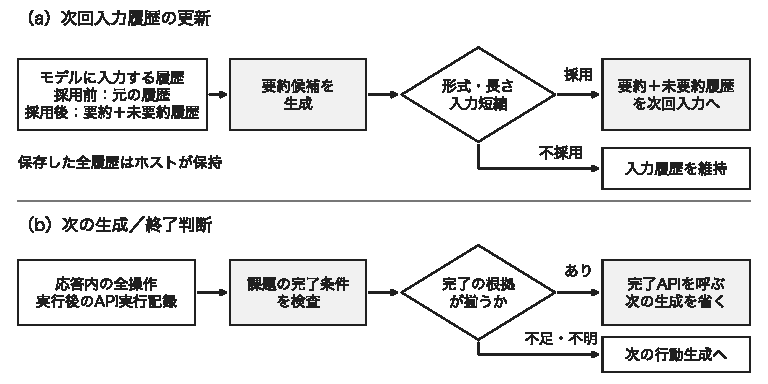
\includegraphics[width=130mm]{figures/control_points.pdf}
\expandafter\def\csname @captype\endcsname{figure}
\capwidth=130mm\ecapwidth=130mm
\abovecaptionskip=4pt\belowcaptionskip=3pt
\caption{履歴要約と終了制御}
\label{fig:architecture}
\end{minipage}\end{center}\vspace{3mm}}]

続いて，形式，文字数，次回actor入力全体の短縮を検査し，全条件を満たす候補だけ採用する．採用時は元の指示と課題を保持したまま，要約と未要約の履歴を次のactorへ渡し，不採用時は従来の提示履歴を維持する．全履歴は保存し続ける．機会回数と閾値は4.1に示し，採否検査は構造と長さを対象とする．

\subsection{API実行記録に基づく終了手順}

既知の1要求文型に対応する手書きの検査規則を用い，終了を判断する．まず，モデル応答内の全プログラムを実行し，APIの要求と応答を記録する．次に，操作前の対象集合と移動前の日時，APIから取得した時刻，対象全件の移動先と元の名前の保持を照合する．これらの照合によって完了の根拠が初めて揃えば完了APIを1回呼び，次の生成を省く．

文型外の操作や，判定に必要な根拠が不確定・矛盾する場合は通常の次生成へ進む．判定には実行中のAPI記録だけを用い，未来応答や公式評価器の正解を参照しない．履歴要約との組合せ効果は評価しない．

\newpage
\begin{samepage}
\subsection{総トークン数と最終成功}

条件$p$で実行したモデル呼出しの集合を$\mathcal C_p$とする．各呼出し$c$の入力トークン数を$I_c$，出力トークン数を$O_c$とし，実行全体の総トークン数$T_p$を\mbox{式\eqref{eq:cost}で求める．}

\begin{equation}
 T_p=\sum_{c\in\mathcal C_p}(I_c+O_c)
 \label{eq:cost}
\end{equation}

集計にはactorとfocusの両方を含め，不採用となった要約の生成や失敗時の呼出しについても，取得できた使用量を計上する．使用量が不明な場合は0とせず，既知分の小計と不明件数を記録する．
\end{samepage}

課題の成功は，実行終了後の状態に対するAppWorld\cite{trivedi2024appworld}の公式評価器で判定する．評価器の正解や詳細は実行中のモデルへ返さない．方式間では成功数と，各課題の成功の維持を確認する．

本指標はキャッシュされた入力も含む論理トークン数であり，金銭課金や実行時間を直接表すものではない\cite{xu2026tokenpilot}．要約生成を含む費用評価はACON\cite{kang2026acon}にも用いられている．実験AとBは独立に集計する．

\section{実験A：要約の呼出し配置}

\subsection{条件}

写真操作，精算，返金，CSV処理の既知4課題に対し，Single，Separate，Inlineの各方式を各課題で1回ずつ実行した（4課題×3方式，計12実行）．全条件は同じMiniMax-M3（GGUF，IQ4\_XS），llama.cpp b11669，文脈長65,536を用いた．モデル生成のseedの基点は57，環境のseedは42で，生成側は呼出しの役割・順序に従いseedを増分した．

要約機会の入力長閾値は16,384トークンとし，要約時には直近2ターンを原文のまま保持する．反復では，前回の要約機会の終了（採否を問わない）から新たに3ターン以上が完了することを要求する．初回の起点は課題開始である．要約機会の上限はSingleが1回，SeparateとInlineが3回である．要約は合計8,192文字以下とし，次のactor入力全体が短くなる場合に採用する．SingleとSeparateのfocus出力上限は4,096トークンで，focusの使用量も式\eqref{eq:cost}へ含める．

各実行の上限はモデル呼出し80回，総トークン数450,000，作業時間1,800秒とし，環境APIは写真160，他3課題80要求とした．actor温度1.0，focus温度0.7，並列実行数1，KV cache q8\_0，計算機はApple M3 Ultra・メモリ256 GiBである．実装と全条件の記録を公開する\footnote{\url{https://github.com/sophiria1225/AI-}}．

\subsection{全4課題の結果}

全4課題の成功を保ち，反復要約のSeparateは単回要約のSingleより総トークン数を107,873（12.07\%）削減した（表\ref{tab:summary}）．全12実行で課題に成功し，使用量の欠測はなく，要約生成を含む課題全体で削減を得た．この差はCSV処理の440,461から332,588への減少によるもので，他の3課題は同じ値だった．

CSV処理での要約採用回数はSingleが1回，SeparateとInlineが各2回だった．写真操作は全方式で1回，精算と返金は0回だった．

\SummaryResultsTable

InlineはSingleより6.34\%少なかったが，Separateより51,266トークン（6.53\%）多かった．Separateとの比較では，写真操作で10,497トークン少ない一方，CSV処理で61,763トークン多かった．要約生成を含む4課題の合計では，Separateが3方式中で最少となった．図\ref{fig:summary}にCSV処理とその他3課題の内訳を示す．

\begin{figure}[!t]
\centering
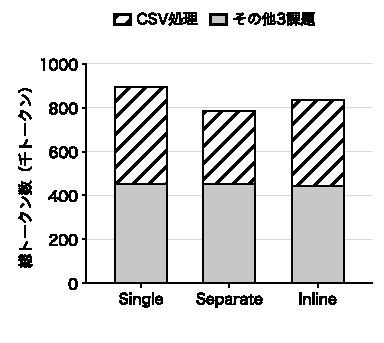
\includegraphics[width=65mm]{figures/result_summary.pdf}
\caption{実験Aの総トークン数}
\label{fig:summary}
\end{figure}

\section{実験B：API実行記録に基づく終了}

\subsection{条件}

同じ写真課題について，API文書の取得を必須とする条件（文書必須）と，公開API名からのアクセスを許す条件（名前参照）を設けた．各APIアクセス条件で，通常継続とAPI実行記録に基づく終了制御（完了判定）を比較した．完了判定は，事前に実行・保存した通常継続と同じ初期状態，モデル，seed，モデルへの指示とツール説明，予算を用いて各1回実行した．

seedの基点は42であり，実験Aとは別の履歴・設定である．同じMiniMax-M3 IQ4\_XSとllama.cpp b11669を用い，各実行の予算はモデル呼出し80回，450,000トークン，1,800秒，API160要求とした．

終了判定と完了通知は3.2に従う．判定，記録保存，完了通知を含む実行時間を記録し，完了通知をAPI要求数に含めた．記録先と集計項目は補足資料\path{EVIDENCE.md}に示す．

\subsection{成功を保った総トークン数の削減}

両API条件で課題の成功を保ち，完了判定により総トークン数を削減した（表\ref{tab:termination}，図\ref{fig:termination}）．文書必須では130,439から91,116へ30.15\%，名前参照では151,664から112,233へ26.00\%減った．全4実行で公式評価器による成功を確認し，使用量の欠測はなかった．各条件でモデル呼出し2回とAPI要求4回を削減した．完了通知を含めて処理を終え，対象の移動後に続いていた4回の確認APIと，それに伴う生成を省いた．

\TerminationResultsTable

実行したAPI操作などの前半の記録と，実行終了時の13個のデータベースのハッシュ値は対照と一致し，最終状態を保った削減を確認した．要求・モデル応答の全文が通常継続側の先頭部分と完全に一致する事前基準は満たさなかったため，結果は既知の要求文型に対する各1回の比較として扱う．平均的な因果効果や汎用的な終了保証を示す評価ではない．

\begin{figure}[!t]
\centering
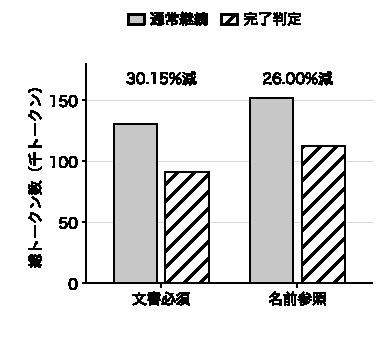
\includegraphics[width=65mm]{figures/result_termination.pdf}
\caption{実験Bの総トークン数}
\label{fig:termination}
\end{figure}

\section{むすび}

既知4課題では，反復要約のSeparateにより全課題の成功を保ち，Singleに比べて総トークン数を12.07\%削減した．同じ写真課題の2つのAPI条件では，API実行記録に基づく完了判定により成功を保ち，通常継続に比べて26.00--30.15\%削減した．要約生成を含む全モデル呼出しを計測し，両制御を独立に評価して実行費用の削減を確認した．

本稿は，既知課題と単一モデル・量子化設定における少数のseed・試行による開発実験を事後に整理した評価である．未見課題の品質維持や統計的非劣性は評価していない．追加条件の採否理由は\path{EVIDENCE.md}に示した．補足の\path{supplemental_results.pdf}と\path{P144R1_all_conditions.csv}には\mbox{全12実行を収録した．}

% Twelve formal conference/journal papers. Source verification: reference_update.json.
\begin{thebibliography}{99}
\bibitem{yao2023react}
S. Yao, J. Zhao, D. Yu, N. Du, I. Shafran, K. Narasimhan, and Y. Cao,
``ReAct: Synergizing reasoning and acting in language models,''
Proc. ICLR, May 2023.

\bibitem{wang2024codeact}
X. Wang, Y. Chen, L. Yuan, Y. Zhang, Y. Li, H. Peng, and H. Ji,
``Executable code actions elicit better LLM agents,''
Proc. ICML, PMLR, vol.235, pp.50208--50232, July 2024.

\bibitem{liu2024lost}
N. F. Liu, K. Lin, J. Hewitt, A. Paranjape, M. Bevilacqua, F. Petroni, and P. Liang,
``Lost in the middle: How language models use long contexts,''
Trans. ACL, vol.12, pp.157--173, 2024.
doi: 10.1162/tacl\_a\_00638.

\bibitem{jiang2023llmlingua}
H. Jiang, Q. Wu, C.-Y. Lin, Y. Yang, and L. Qiu,
``LLMLingua: Compressing prompts for accelerated inference of large language models,''
Proc. EMNLP, pp.13358--13376, Dec. 2023.
doi: 10.18653/v1/2023.emnlp-main.825.

\bibitem{pan2024llmlingua2}
Z. Pan, Q. Wu, H. Jiang, M. Xia, X. Luo, J. Zhang, Q. Lin, V. R\"uhle,
Y. Yang, C.-Y. Lin, H. V. Zhao, L. Qiu, and D. Zhang,
``LLMLingua-2: Data distillation for efficient and faithful task-agnostic prompt compression,''
Findings of ACL: ACL 2024, pp.963--981, Aug. 2024.
doi: 10.18653/v1/2024.findings-acl.57.

\bibitem{jiang2024longllmlingua}
H. Jiang, Q. Wu, X. Luo, D. Li, C.-Y. Lin, Y. Yang, and L. Qiu,
``LongLLMLingua: Accelerating and enhancing LLMs in long context scenarios via prompt compression,''
Proc. ACL, vol.1, pp.1658--1677, Aug. 2024.
doi: 10.18653/v1/2024.acl-long.91.

\bibitem{kang2026acon}
M. Kang, W.-N. Chen, D. Han, H. A. Inan, L. Wutschitz, Y. Chen,
R. Sim, and S. Rajmohan,
``ACON: Optimizing context compression for long-horizon LLM agents,''
Proc. ICML, PMLR, vol.306, pp.55321--55375, July 2026.

\bibitem{xu2026tokenpilot}
B. Xu, Z. Xue, D. Chen, C. Fu, C. Wu, C. Huang, C. Jiang, J. Fang,
X. Deng, Y. Chen, Y. Yao, X. Wang, J. Shang, H. Chen, and N. Zhang,
``TokenPilot: Cache-efficient context management for LLM agents,''
Findings of ACL: EMNLP 2026, pp.19034--19049, Oct. 2026.

\bibitem{park2023generative}
J. S. Park, J. O'Brien, C. J. Cai, M. R. Morris, P. Liang, and M. S. Bernstein,
``Generative agents: Interactive simulacra of human behavior,''
Proc. ACM UIST, article 2, pp.1--22, Oct. 2023.
doi: 10.1145/3586183.3606763.

\bibitem{shinn2023reflexion}
N. Shinn, F. Cassano, A. Gopinath, K. Narasimhan, and S. Yao,
``Reflexion: Language agents with verbal reinforcement learning,''
Advances in Neural Information Processing Systems, vol.36, pp.8634--8652, 2023.
doi: 10.52202/075280-0377.

\bibitem{lu2025runaway}
Q. Lu, L. Ding, S. Cao, X. Liu, K. Zhang, J. Zhang, and D. Tao,
``Runaway is ashamed, but helpful: On the early-exit behavior of large language model-based agents in embodied environments,''
Findings of ACL: EMNLP 2025, pp.24014--24027, Nov. 2025.
doi: 10.18653/v1/2025.findings-emnlp.1304.

\bibitem{trivedi2024appworld}
H. Trivedi, T. Khot, M. Hartmann, R. Manku, V. Dong, E. Li, S. Gupta,
A. Sabharwal, and N. Balasubramanian,
``AppWorld: A controllable world of apps and people for benchmarking interactive coding agents,''
Proc. ACL, vol.1, pp.16022--16076, Aug. 2024.
doi: 10.18653/v1/2024.acl-long.850.

\end{thebibliography}

\end{document}
